% Source-faithful schematic draft: src-6914e1c400640e0c3ef3785cb187876891213e18557a04ba0e97c2f4dae5a999
% Source SHA-256 32093147448a616af26055d81831b7028e661e5138d8546f803a6c6a1a42bc43; PDF p.2, Q21.
% Schematic parameter t=0.4 illustrates AD=t AB, BE=t BC, DM=t DE; this is not an extra value imposed by the source question.
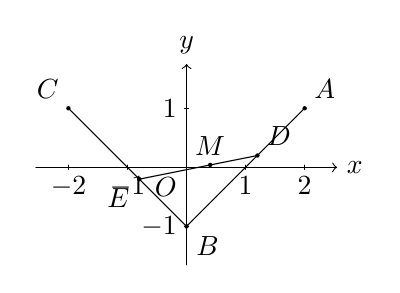
\begin{tikzpicture}[line cap=round, line join=round, x=0.75cm, y=0.75cm]
  \draw[->] (-2.55,0)--(2.55,0) node[right] {$x$};
  \draw[->] (0,-1.65)--(0,1.75) node[above] {$y$};
  \draw (-2,1)--(0,-1)--(2,1);
  \coordinate (A) at (2,1); \coordinate (B) at (0,-1); \coordinate (C) at (-2,1);
  \coordinate (D) at (1.2,0.2); \coordinate (E) at (-0.8,-0.2);
  \coordinate (M) at (0.4,0.04);
  \draw (D)--(E);
  \foreach \P/\label/\pos in {A/A/above right,B/B/below right,C/C/above left,D/D/above right,E/E/below left,M/M/above} {
    \fill (\P) circle (0.8pt) node[\pos] {$\label$};
  }
  \node[below left] at (0,0) {$O$};
  \foreach \xv in {-2,-1,1,2} {\draw (\xv,0.035)--(\xv,-0.035);}
  \foreach \yv in {-1,1} {\draw (0.035,\yv)--(-0.035,\yv);}
  \node[below] at (-2,0) {$-2$}; \node[below] at (-1,0) {$-1$};
  \node[below] at (1,0) {$1$}; \node[below] at (2,0) {$2$};
  \node[left] at (0,1) {$1$}; \node[left] at (0,-1) {$-1$};
\end{tikzpicture}
